\let\negmedspace\undefined
\let\negthickspace\undefined
\documentclass[journal]{IEEEtran}
\usepackage[a5paper, margin=10mm, onecolumn]{geometry}
%\usepackage{lmodern} % Ensure lmodern is loaded for pdflatex
\usepackage{tfrupee} % Include tfrupee package

\setlength{\headheight}{1cm} % Set the height of the header box
\setlength{\headsep}{0mm}     % Set the distance between the header box and the top of the text

\usepackage{gvv-book}
\usepackage{gvv}
\usepackage{cite}
\usepackage{amsmath,amssymb,amsfonts,amsthm}
\usepackage{algorithmic}
\usepackage{graphicx}
\usepackage{textcomp}
\usepackage{xcolor}
\usepackage{txfonts}
\usepackage{listings}
\usepackage{enumitem}
\usepackage{mathtools}
\usepackage{gensymb}
\usepackage{comment}
\usepackage[breaklinks=true]{hyperref}
\usepackage{tkz-euclide} 
\usepackage{listings}
% \usepackage{gvv}                                        
\def\inputGnumericTable{}                                 
\usepackage[latin1]{inputenc}                                
\usepackage{color}                                            
\usepackage{array}                                            
\usepackage{longtable}                                       
\usepackage{calc}                                             
\usepackage{multirow}                                         
\usepackage{hhline}                                           
\usepackage{ifthen}                                           
\usepackage{lscape}
\usepackage{circuitikz}
\tikzstyle{block} = [rectangle, draw, fill=blue!20, 
    text width=4em, text centered, rounded corners, minimum height=3em]
\tikzstyle{sum} = [draw, fill=blue!10, circle, minimum size=1cm, node distance=1.5cm]
\tikzstyle{input} = [coordinate]
\tikzstyle{output} = [coordinate]


\begin{document}

\bibliographystyle{IEEEtran}
\vspace{3cm}

\title{1.9.2}
\author{EE25BTECH11013 - Bhargav}
\maketitle
% \newpage
% \bigskip
{\let\newpage\relax\maketitle}

\renewcommand{\thefigure}{\theenumi}
\renewcommand{\thetable}{\theenumi}
\setlength{\intextsep}{10pt} % Space between text and floats


\numberwithin{equation}{enumi}
\numberwithin{figure}{enumi}
\renewcommand{\thetable}{\theenumi}

\textbf{Question}:\\
The point on the X axis which is equidistant from \brak{-4,0} and \brak{10,0} is\\ 
\solution \\
Let the 2 points be $\vec{A}$ and $\vec{B}$ and let the desired point equidistant from both $\vec{A}$ and $\vec{B}$ be $\vec{O}$:
\begin{align}
\vec{A}=\myvec{-4 \\ 0},\quad
\end{align}
\begin{align}
\vec{B}=\myvec{10 \\ 0},\quad
\end{align}
\begin{align}
\vec{O} = x\,\mathbf e_1= \myvec{$x$ \\ $0$}
\end{align}
If $\vec{O}$ lies on $X$ axis and is equidistant from $\vec{A}$ and $\vec{B}$



\begin{align}
\|\vec{O}-\vec{A}\|=\|\vec{O}-\vec{B}\|
\end{align}

\begin{align}
\implies \|\vec{O}-\vec{A}\|^2 = \|\vec{O}-\vec{B}\|^2
\end{align}

\begin{align}
\implies (\vec{O}-\vec{A})^{\top}(\vec{O}-\vec{A}) = (\vec{O}-\vec{B})^{\top}(\vec{O}-\vec{B})
\end{align}

\begin{align}
\implies \vec{O}^{\top}\vec{O} - 2\vec{O}^{\top}\vec{A} + \vec{A}^{\top}\vec{A}
= \vec{O}^{\top}\vec{O} - 2\vec{O}^{\top}\vec{B} + \vec{B}^{\top}\vec{B}
\end{align}


\begin{align}
\implies \|\vec{O}\|^2 - 2\vec{O}^{\top}\vec{A} + \|\vec{A}\|^2
= \|\vec{O}\|^2 - 2\vec{O}^{\top}\vec{B} + \|\vec{B}\|^2
\end{align}
\begin{align}
    (\vec{A}-\vec{B})^{\top}\vec{O}=\frac{\|\vec{A}\|^2-\|\vec{B}\|^2}{2}.
\end{align}

\begin{align}
     \vec{O} = x \mathbf{e}_1,
\end{align}

\begin{align}
    x = \frac{\|\vec{A}\|^2 - \|\vec{B}\|^2}{2 (\vec{A} - \vec{B})^{\top} \mathbf{e}_1}.
\end{align}

Solving for $x$, we get $x$ = $3$\\

\begin{align}
    \therefore \vec{O} = \myvec{$3$ \\ $0$}
\end{align}
\begin{figure}[h!]
    \centering
    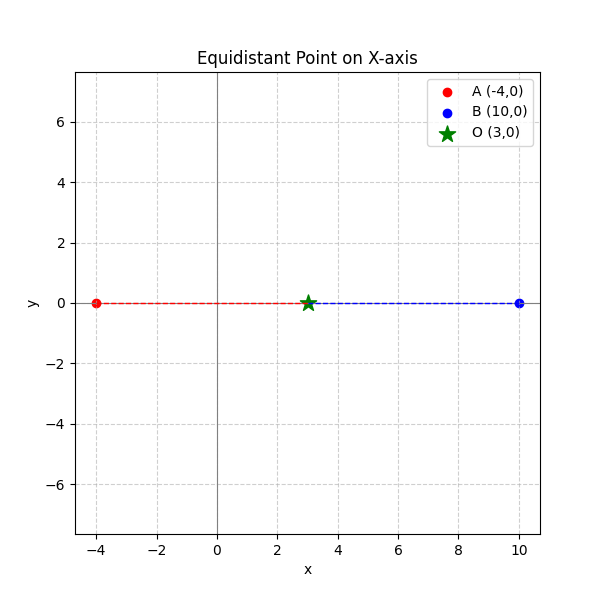
\includegraphics[height=0.5\textheight, keepaspectratio]{figs/Figure_1.png}
    \label{figure_1}
\end{figure}



\end{document}


